\section{CCA\hpoints{13}}

Canonical correlation analysis (CCA) is a method similar to PCA, but
instead of finding the directions of maximum variance (or minimum reconstruction error) within a matrix,
it handles the situation that each data point (i.e., each observation) has two
representations (i.e., two sets of features or ``views''), e.g., a web page can be
represented by the text on that page, and can also be represented by
other pages linked to that page. 

As a simple example, assume each data point has two
representations $x$ and $y$, each of which is a 2-dimensional feature
vector, i.e., $x = [x_1; x_2]^T$ and $y = [y_1; y_2]^T$. Note that in general $x$ and $y$ can have different
numbers of features in them. Given a set of data
points, CCA finds a pair of projection directions $(u; v)$ to maximize the
sample correlation $corr[(u^T x),(v^T y)]$ along the directions $u$ and $v$. In
other words, after we project the $x's$ onto $u$
and the $y's$ onto  $v$, the two projected
representations $u^T x$ and $v^T y$ should be maximally correlated.
Intuitively, data points with large values in one projected direction
should also have large values in the other projected direction.

\begin{enumerate}
\item \points{5} 
Consider the data points shown in the figure below. 
The data $x$ and $y$ are paired -- each point in the left figure corresponds to a specific point in the right figure and vice versa, since these two points are two representations (views) of the same object. 
Different objects are shown in different gray scales in the two figures (so you should be
able to approximately figure out how points are paired). In the right figure we've given one CCA projection
direction $v$, draw the other CCA projection direction $u$ in the left figure. (Problem adapted from Yi Zhang at CMU.)

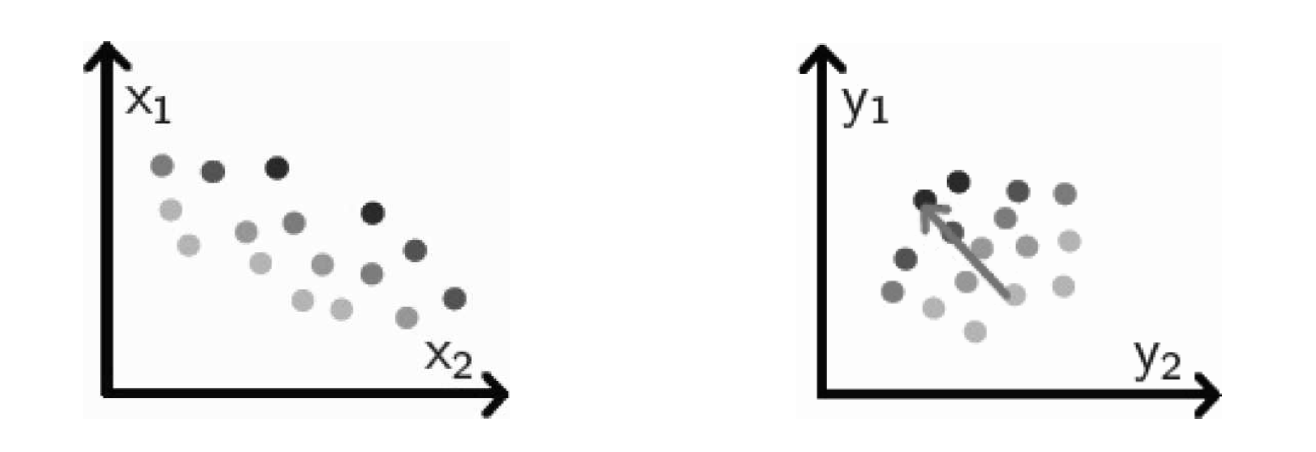
\includegraphics[width=0.6\textwidth]{images/cca.png}


\item \points{8} 
The formal solution for CCA is that the projections $U$ and $V$ are the (largest) left and right singular vectors of
$Z=(X^TX)^{-1/2} X^TY (Y^TY)^{-1/2}$ where $X$ and $Y$ are the two ``views'' of the data, each containing $n$ observations. 
Using the breast cancer data in \(\mathtt{breast\_cancer.mat}\), define \(\mathtt{X=X\_train}\) and \(\mathtt{Y=Y\_train}\) and compute the single largest left and right singular vectors for the matrix \(Z\) as described above.
These are the ``canonical vectors'' .
Here, $X$ is of dimension $n \times p_x$, $Y$ of dimension $n \times p_y$,
$U$ of dimension $p_x \times k$, and $V^T$ of dimension $p_y \times k$.  Since we keep only one (largest) component, $k=1$ in this case.


\begin{enumerate}
\item What is the correlation between  $XU$ and $YV^T$? 
This asks how correlated the two different estimates of the 'hidden state' from the two views are. 
CCA tries to make this number as big as possible.
Note that in this problem  we are looking at the ``degenerate'' case which the $y$ view has only a single feature.

\item How does the above compare to the correlation between $\hat{y}$ and $y$ where 
$\hat{y}$ is this the result of estimating $y$ using only a single principle component, i.e. principle components regression (PCR) with a single component.

%(e.g., as done with $k=1$ on the previous problem.

\end{enumerate}


\end{enumerate}
